\chapter{Rover Implementation}
\lhead{\emph{Rover Implementation}}
\label{chapter:rover}

The aim of this project is the development of a VR teleoperations system. This necessitates the procurement of some form of robotic platform to demonstrate the system on. This platform must be easily modifiable and cheap enough to be within budget, so it was determined that the most logical solution was to design a simple rover for the project; this is both cheap and allows for complete customisation with minimal hassle. The internals of the rover are shown in Figure \ref{fig:internals}, and a block diagram of the hardware in Figure \ref{fig:hardware}.

\begin{figure}[H]
    \begin{center}
    \begin{tabular}{ c c }
        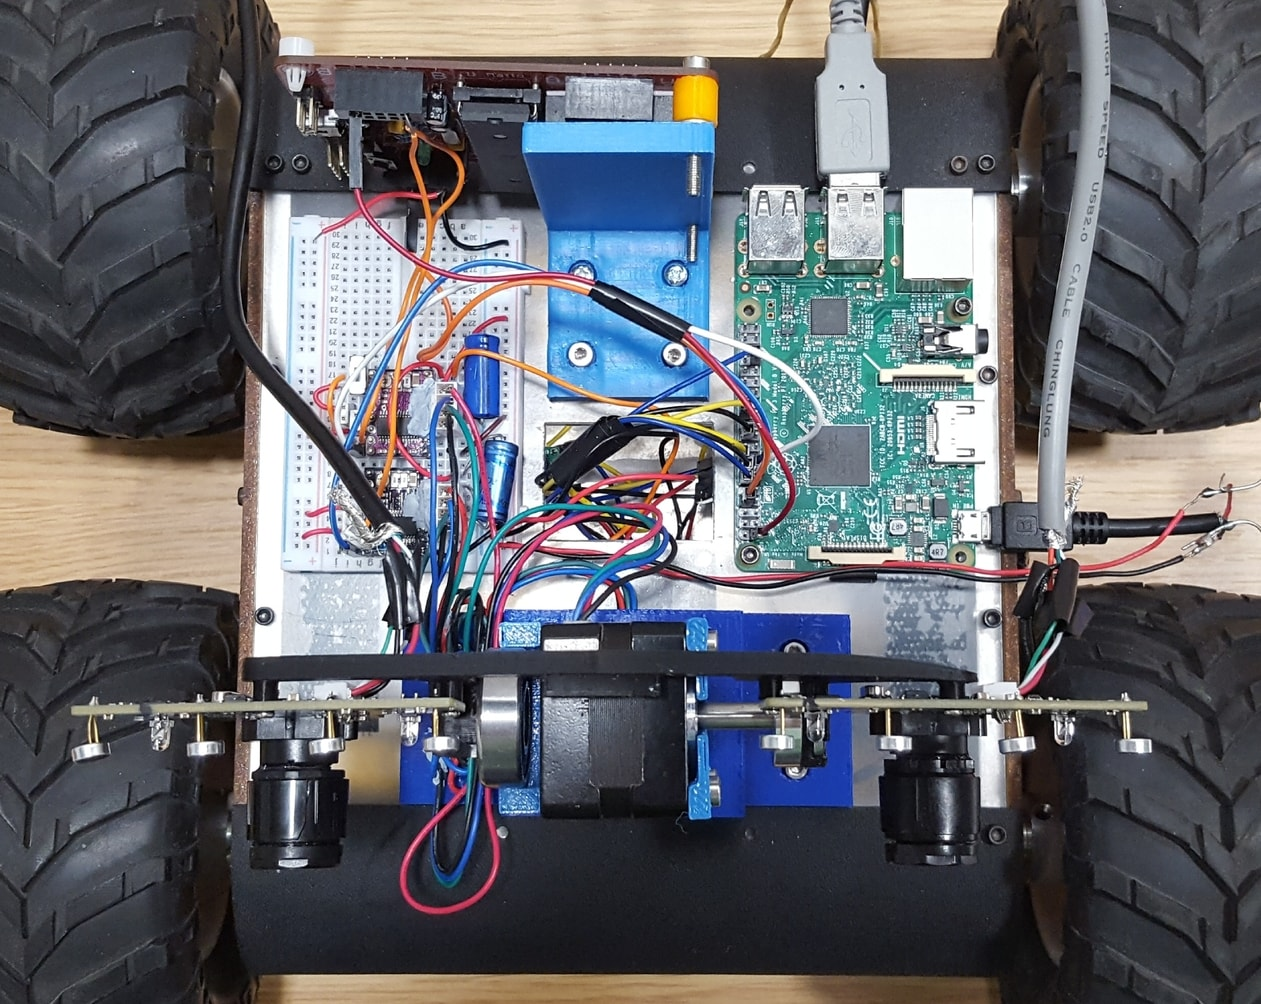
\includegraphics[width=0.47\textwidth]{Figures/rovertop.jpg} &
        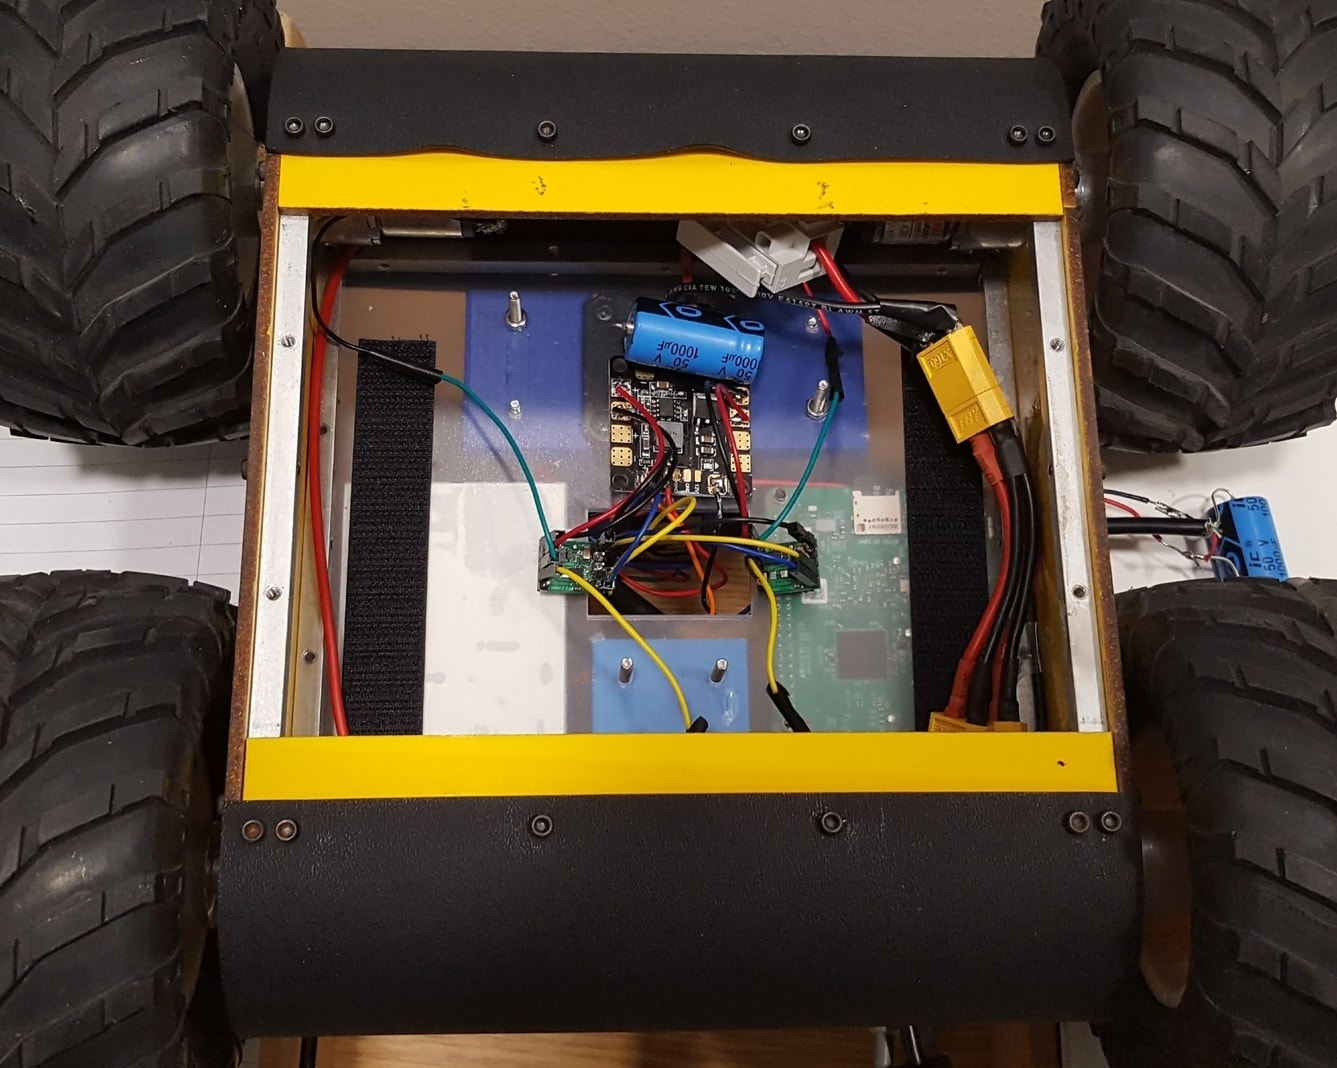
\includegraphics[width=0.47\textwidth]{Figures/roverinside.jpg}
    \end{tabular}
    \caption[Rover Internals]{Rover Internals. The left picture is a top-down view of rover, in which you can see the Pi on the right, the Il Matto mounted vertically at the top, the gimble at the bottom, and the stepper motor drivers for the gimble on the breadboard on the left. The right picture is of the inside of the rover, taken through a hatch in its underside. In this picture you can see velcro strips marking where the batteries are attached, a power distribution board and fuse in the centre, 2 DC motor drivers just below that, and 2 of the 4 DC motors in the top corners.}
    \label{fig:internals}
    \end{center}
\end{figure}

 Due to the rover being a simple test platform for the proposed system, its hardware is mostly irrelevant to this report and therefore will not be discussed in detail (a detailed breakdown can be found in Appendix \ref{appendix:hardware}). The application of computer vision techniques in an embedded system has high processing requirements, leading to the selection of a Raspberry Pi 3 as the core of the system (it was the highest performance embedded device readily available). 

\begin{figure}[H]
    \begin{center}
      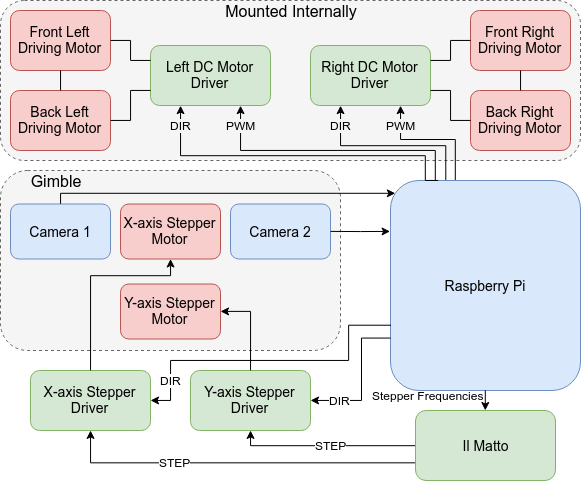
\includegraphics[width=0.9\textwidth]{Figures/hardware.png}
      \caption[Hardware Block Diagram]{Hardware Block Diagram. The red blocks are motors, green blocks are control system components, and the blue blocks are part of the image pipeline.}
      \label{fig:hardware}
    \end{center}
\end{figure}

\section{Gimble Design}

The choice of cameras had to fulfil a very specific set of requirements. The two cameras must be same, as any differences in the images due to the cameras would reduce the quality of depth map produced by the block matching algorithm on the server. This makes the most obvious camera choice, the R-Pi camera module, unusable, as the Pi cannot use two simultaneously. The two cameras must also be able to take pictures on command from the Pi with low latency, reducing the possible options down to primarily USB webcams. Finally, they must have a high shutter speed. Any motion blur in the images will blur all the edges they contain, making them undetectable by the edge detection algorithm, and any morphing of the image while under motion due to the time it takes the shutter to pass across the entire sensor will once again reduce the quality of the depth map; a high shutter speed reduces motion blur and shutter related morphing, therefore making it essential for whenever the rover is in motion. This requirement reduces the possible cameras down to primarily dedicated computer vision cameras, however these are far outside the budget of a 3rd year project and are often too large to build a gimble for without also buying expensive motors.

\textcolor{red}{[FPV CAMERA APPENDIX?]}

Only one camera was found that fulfilled all these requirements while being cheap enough to fit within budget- the PlayStation 3 (PS3) Eye. The PS3 Eye is a camera for the PS3 to allow for games that incorporate aspects of computer vision, so it is designed with computer vision and value for money in mind. While the image quality is fairly poor, it is sufficient for the system to function reliably. 

The design of the gimble (Figure \ref{fig:gimble}) has considerable impact on the 3D environment the system produces. As mentioned in Section \ref{subsection:depth}, the closer the cameras are to parallel with each other, the less the images have to be rectified before the depth map is generated. Similarly, the stability of the gimble is very important, as any vibrations will cause inconsistency in the alignment of the cameras, leading to inaccurate depth maps. This led to the chosen design where the X-axis motor is located centrally, between the cameras, to balance the weight around the rotational axis of the y-axis motor. The 3D-printed part the cameras are attached to is also stabilised through mountings on both sides of the x-axis motor, using a ball bearing on the side not driven by the motor. 

\begin{figure}[H]
    \begin{center}
      \includegraphics[width=0.7\textwidth]{Figures/gimble.jpg}
      \caption[Gimble Picture]{Gimble Picture. The Y-axis motor is housed at the bottom, with the X-axis motor directly above it. The ball bearing that stabilises the non-driven side of the cameras' backplate can be seen to the left of the X-axis motor.}
      \label{fig:gimble}
    \end{center}
\end{figure}

Another important aspect of the gimble design is the distance between the camera lenses. The further apart the two cameras are, the closer distance objects will be in the depth map. Ideally we would want to match the interpupillary distance of human eyes (63mm on average \cite{dodgson2004variation}), so objects in the 3D environment appear as close as they would were the user standing in the place of the robot. However, with the X-axis motor located centrally, it is not possible to produce that distance between the camera lenses. The inter-lens distance in the final design is 120mm, as this is the closest distance possible without reducing the stability of the gimble. While not ideal, it simply results in objects appearing closer in the depth map than they actually are and a longer distance from the cameras where an object is too close for a distance to be calculated (the cameras are "cross-eyed" if you will).

\section{Image Pipeline}
\label{Subsection:comms}

As can be seen in Figure \ref{fig:system}, the rover takes a picture with both cameras, abstracts those images, then sends that data off as a single combined packet to the server. While Chapter \ref{chapter:abstract} discussed the abstraction process as a single step that produces a full abstraction with both edges and spaces filled with colour, this does not reflect the implementation utilized in the full system. As previously mentioned, the final step of filling the spaces in the edge detected image using the selected seed points and average colours is done on the server. Also, only one of the two images needs colour information at all, as the edges are the only part of the abstraction required to produce the server depth maps; the colours are to be used as a texture on the 3D environment this produces, and therefore only one set is required. Therefore, the data packets being sent to the server are made up of 2 bitmaps of the edge detected images and a set of seed points with their corresponding colours for one of the images.

Attempts to implement this process on a single thread on the Pi, as tested successfully on a laptop, either crashed the Pi or would produce a frame rate of around 1fps; the Pi's resources are not even close to adequate. To combat this, both pipelining and parallelism were utilized to make better use of the Pi's quad core processor (Figure \ref{fig:threads}), and compromises were made in the quality of the abstractions to reduce the workload.

The capture thread simply handles signalling the cameras to take a picture each. The capture and decoding of the images are done as separate operations to make the capture operation shorter and therefore the two cameras capturing as close to simultaneously as possible with a single thread. The first compromise in quality in favour of performance is made here, where the images are captured with a resolution of 320x240 rather than the cameras' standard resolution of 640x480. As will be discussed in greater depth later in this section, the highest workload task in the pipeline is flood filling. It can therefore be inferred that reducing the pixel count of every space by a factor of four would have provide a significant improvement in performance. The smaller images also have the benefit of lower detail in high detail areas, so sections that would become areas of dense lines when edge detected (examples of this effect can be found in Appendix \ref{Appendix:demo}) will be significantly less dense, containing less extraneous data.

\begin{figure}[H]
    \begin{center}
      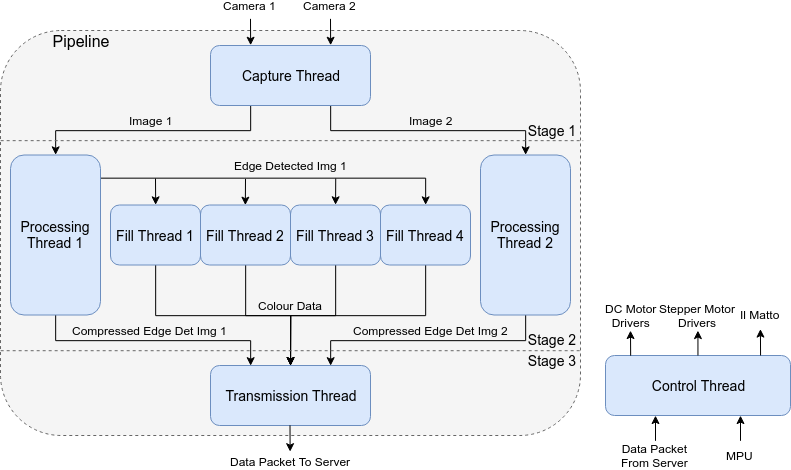
\includegraphics[width=1\textwidth]{Figures/Threads.png}
      \caption[Raspberry Pi Threading Block Diagram]{Raspberry Pi Threading Block Diagram.}
      \label{fig:threads}
    \end{center}
\end{figure}

The processing threads are concerned with the edge detection and compression of the images. The edge detection process is mostly as described in Chapter \ref{chapter:abstract}; the only difference is only the image being sent from processing thread 1 to the fill threads undergoes the final dilation step. The purpose of the dilation is to bridge gaps between the edges, creating defined shapes for the flood fill process. A side effect of dilation is a reduction in edge accuracy, which is very important when the images are to be used to produce depth maps later on. This leads to the logical conclusion that the images should be sent without dilation, and dilation only applied to find the colour data in the fill threads and then again on the server to create the complete coloured abstraction, allowing the depth maps to be constructed with non-dilated images. 

While it can be induced from comparing the original images to their edge detected versions by eye that the latter contains less information than the former, this will only be reflected in real numbers if file format and compression are considered carefully. When the common image formats are compared, PNG would appear to be effective for this use case \cite{aguilera2006comparison}, as it excels at efficiently storing large blocks of the same colour (most of each edge detected image is black space). When tested on the edge detected images (Figure \textcolor{red}{[COMPRESSION COMPARISON]}), it was confirmed that PNG provided the lowest file size, and compression level 5 provided the best ratio between file size and compression time (using the imencode function in OpenCV). More intelligent compression was tested using libimagequant \cite{libimagequant}, however it resulted in very poor performance (\textless2fps) with negligible improvement to the level of compression. An alternate option to compression as a bitmap was vectorising the images, however this was inaccurate and not as effective as bitmap compression (more information can be found in Appendix \ref{appendix:vectorization}).

As previously established, the stage in the image pipeline that has the highest performance impact is the colour averaging, due to its use of flood filling. As the number of spaces being flood filled is determined by the number of points from the sobol sequence being sampled, the number of sobol points is an important variable in tuning the performance of the system. In the testing done on a laptop in Chapter \ref{chapter:abstract}, the number of sobol points being used per image was always between 400 and 600, and this filled a reasonable number of spaces while providing a reasonable frame rate of \textcolor{red}{[REDO FPS TESTS]}. When this was attempted on the Pi however, the frame rate was significantly below 1fps. This called for a significant reduction in sobol points and the application of parallelism; good performance was achieved using 4 threads dedicated to the flood fill colour averaging task, each taking 15 sobol points. A total of 60 sobol points is a significant reduction from the laptop implementation of the algorithm, however it must also be noted that the images being used are much smaller, so do not require a large number of sobol points to have been mostly covered (Figure \textcolor{red}{[ROVER/LAPTOP ABSTRACTION COMPARISON]}). While it may seem as though the parallelization of this process could cause issues if two threads are attempting to fill the same space in the image simultaneously, this simply results in two successful seed points with slightly inaccurate average colours assigned to them, and only one of them being used to create the complete abstraction on the server. As the colours of the spaces are only recorded to provide the user a better understanding of the objects in the environment, it is not concerning if occasionally one is not an exact average.

Once the three pieces of data for an image pair (two compressed edge detected images and a set of colour data) have been generated, they must be combined into a single packet and sent to the server; this is covered by the transmission thread. While the images are at this stage already compressed into a set of bytes that can be transmitted as is, the colour data needs its own custom packaging. Each seed point-average colour pair is formed into its own sub-packet with the structure shown in Table \ref{table:colour}. These sub-packets make up the colour data data segment within the complete data packet.

\begin{table}[H]
\centering
\caption{Colour Data Sub-Packet Structure. The seed point components are given 2 bytes each due to their maximum values being larger than a single byte can store.}
\label{table:colour}
\begin{tabular}{|c|c|c|c|c|c|c|c|}
\hline
Byte in Colour Data Sub-Packet & 1          & 2         & 3          & 4         & 5         & 6           & 7         \\ \hline
Usage                          & \multicolumn{4}{c|}{Seed Point}                 & \multicolumn{3}{c|}{Average Colour} \\ \hline
Component                      & \multicolumn{2}{c|}{X} & \multicolumn{2}{c|}{Y} & Red       & Green       & Blue      \\ \hline
\end{tabular}
\end{table}

As the size of each data segment is unknown and highly variable, knowing where one ends and another begins on the server is a challenge. The solution utilized in this instance is separating each data set with a splitter made up of 7 bytes that contain 0, 1, 2, 3, 4, 5, and 6. This sequence of bytes is extremely unlikely to occur within the data, so can be easily used to pinpoint the starts and ends of the data sets. This therefore leads to the data packet format shown in Table \ref{table:packet}.

\begin{table}[H]
\centering
\caption{Data Packet Format.}
\label{table:packet}
\resizebox{\textwidth}{!}{
\begin{tabular}{|c|c|c|c|c|c|c|c|}
\hline
Data Segment & \multicolumn{3}{c|}{Colour Data}  & Splitter & Img 1          & Splitter & Img 2          \\ \hline
Contents     & Sub-Packet 1 & Sub-Packet 2 & ... & 0...6    & PNG Data & 0...6    & PNG Data \\ \hline
\end{tabular}}
\end{table}

\section{Control System}

Xbox controls

Data packet format

PID loop